% !TEX root = \linearpartition.tex

% state the problem
% RNA secondary structure prediction is a well-known problem, and it has been used for medical design. 
% Compared with MFE-based methods, partition function-based methods attract more and more attention due to their higher accuracy and ability to predict pseudoknots.
% Recently, 
% For example, almost every week a new ncRNA is found to be regulated in a particular disease, or a new class of noncoding
% transcripts is uncovered by a transcriptomic study, or a new
% article heralds a paradigm shift that lncRNAs will bring to
% our understanding of biology 
% Each year, noncoding RNA 
% Ribonucleic acid (RNA) 

\section{Introduction}

% \begin{figure}[t]
% \center
% \begin{tabular}{cc}
% \hspace{-3cm}\panel{A} & \hspace{-3cm}\panel{B} \\
% 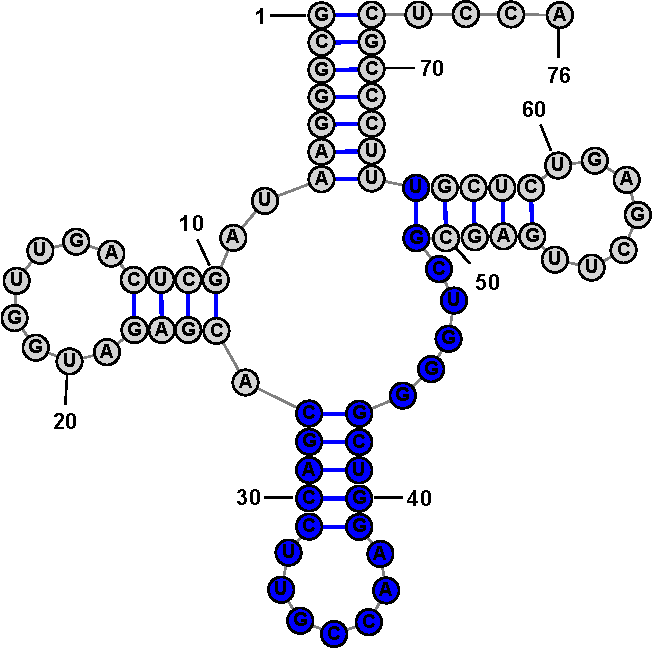
\includegraphics[scale=0.3]{figs/gold_RNAstructure}
% &
% 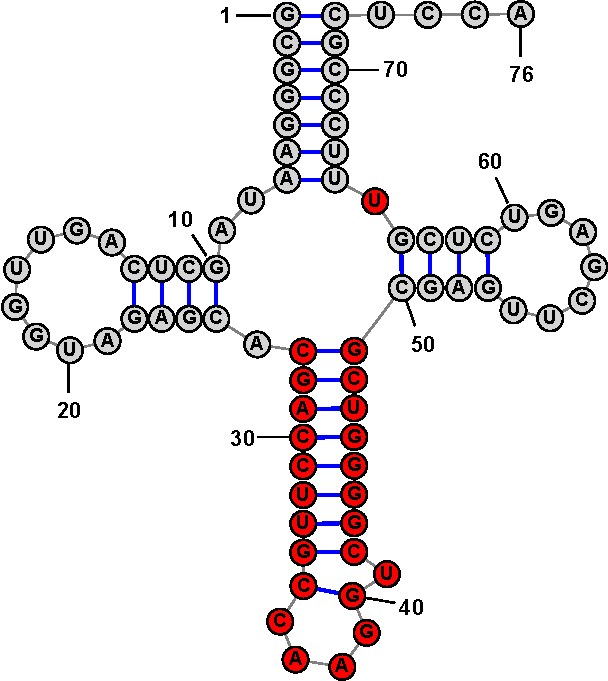
\includegraphics[scale=0.3]{figs/mfe_RNAstructure}\\
% \hspace{-3cm}\panel{C} & \hspace{-3cm}\panel{D}\\[-0.4cm]
% 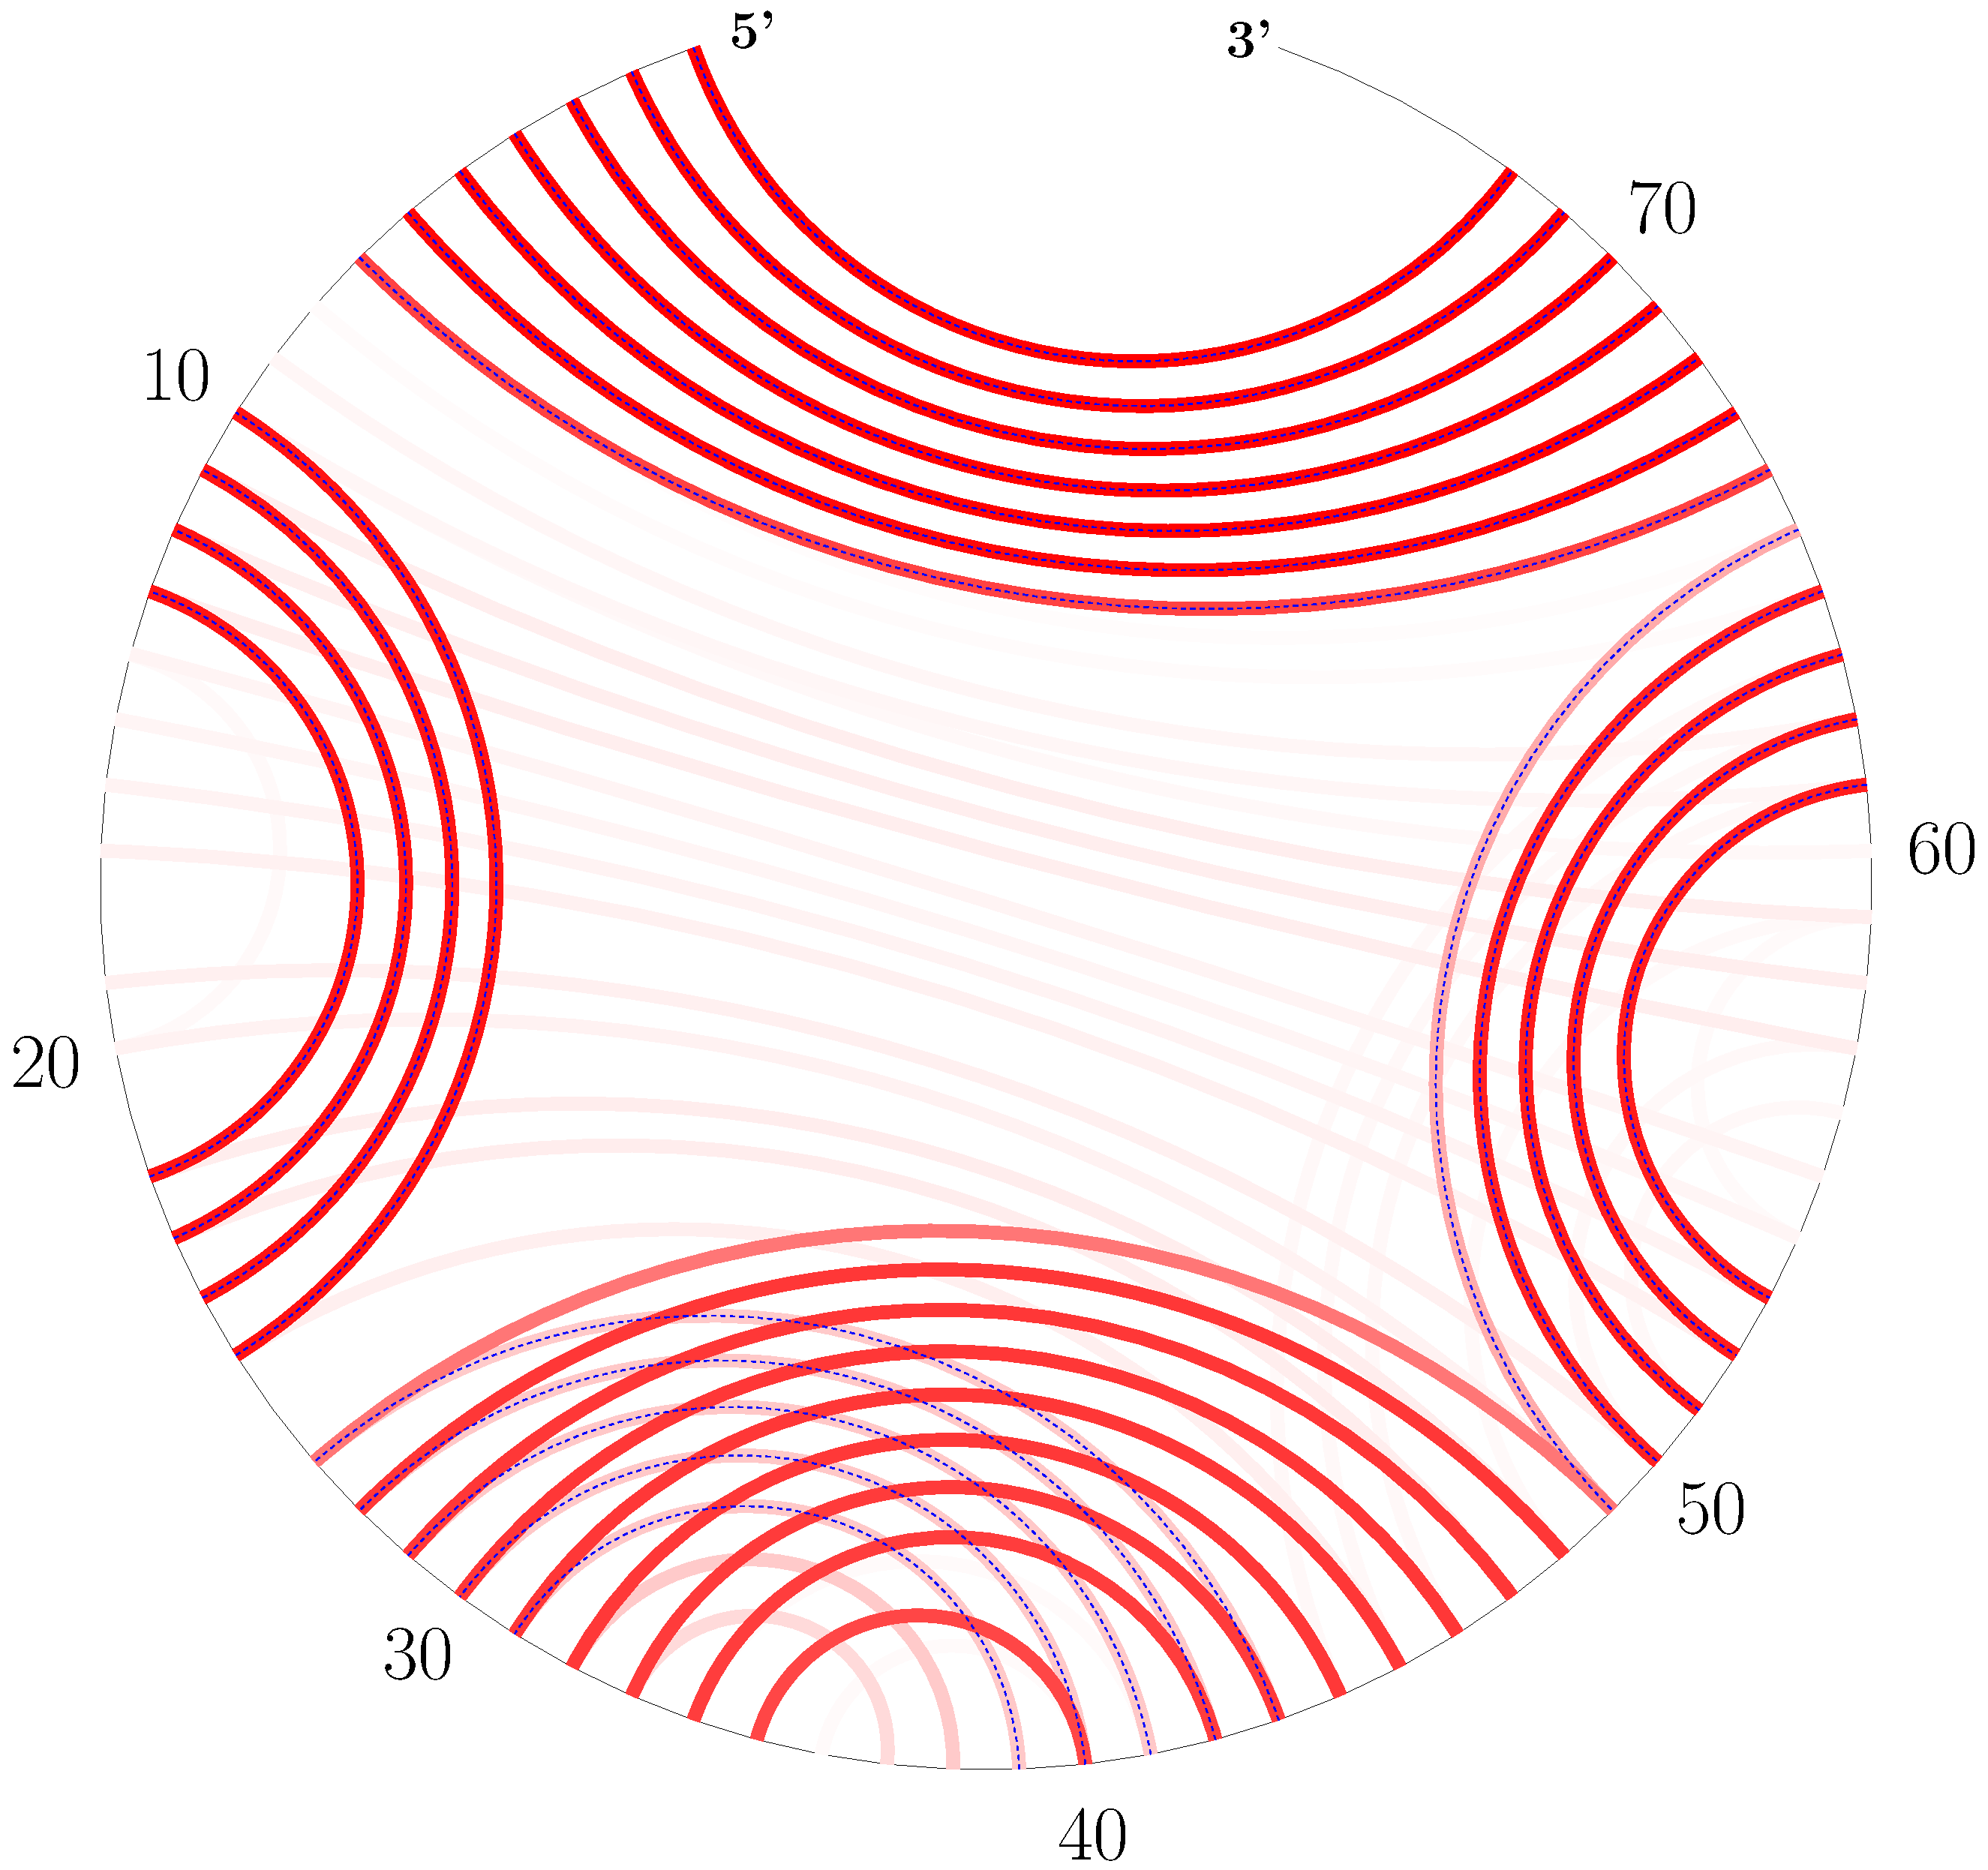
\includegraphics[scale=0.085]{figs/tRNA_circular}
% &
% 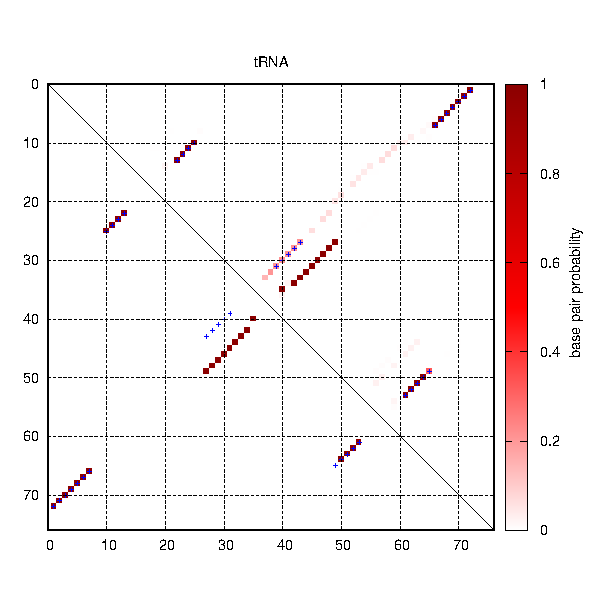
\includegraphics[scale=0.4]{figs/tRNA_heatmap_dark}

% \end{tabular}
% \caption{
% Comparison of MFE-based method and partition function-based method. 
%     {\bf A}: ground truth secondary structure of {\it E.~coli} tRNA$^\textit{Gly}$; 
%     {\bf B}: the corresponding MFE structure. 
%     Structural difference are denoted with blue in ground truth structure and red in MFE structure;
%     {\bf C}: the corresponding circular representation.
%     Ground truth base pairs are denoted with dash blue lines. 
%     Base pair probabilities are denoted with red solid lines and line shade is proportional to probability value.
%     {\bf D}: the corresponding heatmap representation.
%     MFE structure (lower triangle) misses some ground truth base pairs (blue cross), 
%     while base pairing probability matrix (upper triangle) covers these correct base pairs. 
% \label{tRNA}}
% \end{figure}

\begin{figure}[t]
\center
\begin{tabular}{cc}
% \hspace{-3cm}\panel{A} & \\[-0.6cm]
% % \\[-0.6cm]
% \multicolumn{2}{c}{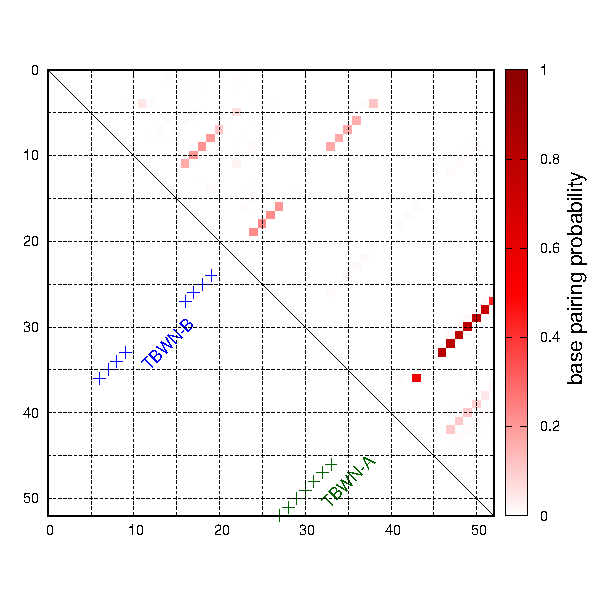
\includegraphics[scale=0.7]{figs/heatmap_fig1A}}
\\[-0.7cm]
\raisebox{6.5cm}{\hspace{-3.5cm}\panel{A}} & \hspace{-4cm}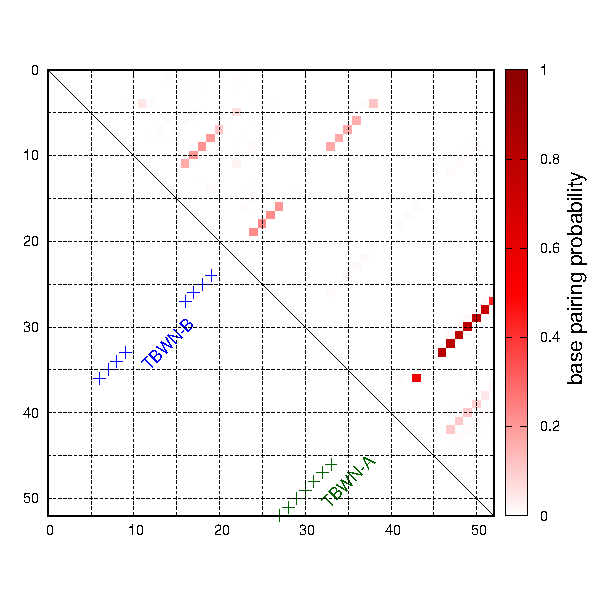
\includegraphics[scale=0.75]{figs/heatmap_fig1A}
\\[-0.2cm]
\hspace{-1cm}\panel{B} & \hspace{2cm}\panel{C}\\[-0.4cm]
\hspace{-0.5cm}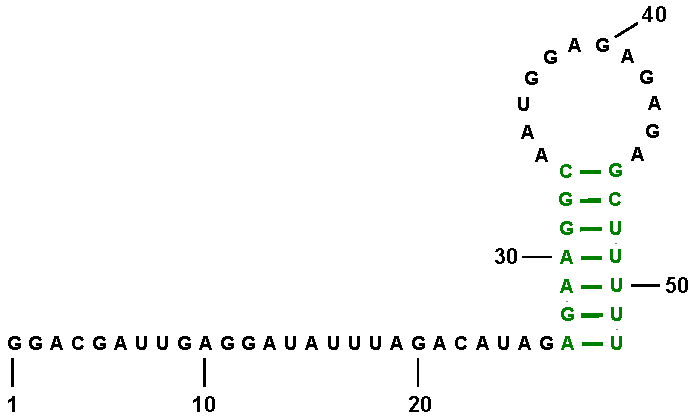
\includegraphics[scale=0.35]{figs/TBWN-A-2}
&\hspace{0.1cm}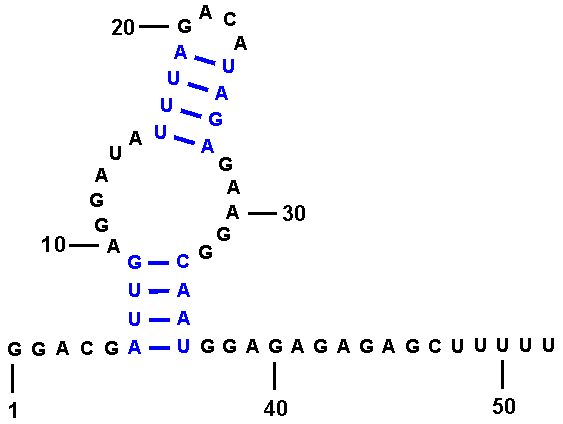
\includegraphics[scale=0.35]{figs/TBWN-B-3}\\
% 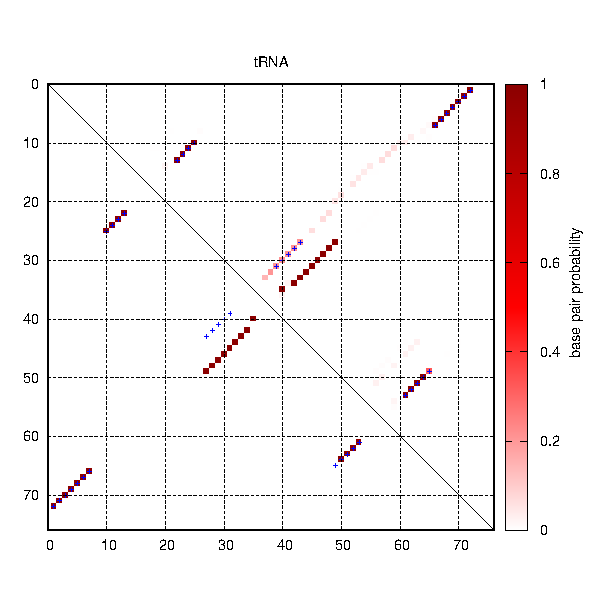
\includegraphics[scale=0.4]{figs/tRNA_heatmap_dark}
\end{tabular}
\caption{
An example of Tebowned RNA illustrates 
% some RNAs 
an RNA that
folds into more than one structure at equilibrium~\cite{Cordero+Das:2015}.
	{\bf A}: upper triangle shows the estimated base pairing probability matrix for Tebowned RNA, and dark red squares represent high probility base pairs; the lower triangle shows two different structures of Tebowned RNA at equilibrim, green crosses for TBWN-A and blue crosses for TBWN-B base pairs;
    {\bf B}: TBWN-A secondary structure;
    {\bf C}: TBWN-B secondary structure.
\label{Tebowned-RNA}}
\vspace{-0.3cm}
\end{figure}

% For past decades, our understanding of ribonucleic acid (RNA) is changing. 
% New proofs reveal that 
% noncoding 
% RNAs %(ncRNAs) 
% Ribonucleic acids (RNAs)
RNAs
are involved in multiple processes, 
such as catalyzing reactions or guiding RNA modifications~\cite{Eddy:2001,Doudna+Cech:2002,Bachellerie+:2002}, 
% and regulating a particular disease~\cite{Kung+:2013},
and their functionalities are highly related to structures.
% but determining the structure using experimental methods is costly and time-comsuming. 
%%%%%%%%5
% from proposal
% Therefore, being able to %rapidly 
% determine the structure is %extremely 
% useful and desired.
% given the overwhelming pace of increase in genomic data (about 1021 base-pairs per year \cite{stephens+:2015}) %[97] 
% and given the small percentage of sequences that have experimentally determined structure. 
% While experimental assays still constitute the most reliable way to determine structures, they are prohibitively costly, slow, and difficult.
However, 
% both 
structure determination techniques, such as X-ray crystallography~\cite{Kim+:1971} 
or Nuclear Magnetic Resonance (NMR)~\cite{Scott+Hennig:2008}, 
and 
% chemical probing methods 
cryo-electron microscopy~\cite{Lyumkis:2019}, 
% ~\cite{Ziehler+Engelke:2001},
though reliable and accurate,
are extremely slow and costly.
% considering the exponentially increasing genomic data (about $10^{21}$ base-pairs per year \cite{stephens+:2015}) 
% and undetermined structures.
% and therefore computational prediction provides an attractive alternative.
%%%%%%%%%%%%
% Due to such limitations, fast and accurate RNA structure prediction is required and desired,
% Due to such limitations, 
% for many RNA tasks 
Therefore,
fast and accurate computational prediction of RNA structure is useful and desired. %required. 
Considering full RNA %tertiary 
structure prediction is challenging~\cite{Miao+:2017},
% \cite{mccaskill:1990},
% even more difficult than protein folding \cite{mccaskill:1990},
% as an alternative
many studies focus on predicting secondary structure,
% the double helices folding structure formed by self-complementary nucleotides
the set of canonical base pairs in the structure 
(A-U, G-C, G-U base pairs)~\cite{Tinoco+Bustamante:1999},
% RNA secondary structure prediction
as it is well-defined, 
% in mathematics formation, 
and provides detailed information to help understand 
% RNA's mechanism of functionality,
the structure-function relationship.
% functionality 
% as well as further 
The secondary structure additionally is a basis to predict full tertiary structure
~\cite{Flores+Altman:2010,Seetin+Mathews:2011}.
% ~\cite{Flores+Altman:2010,Seetin+Mathews:2011tinoco+:1971, auron+:1982}.

\begin{figure}[h]
\center
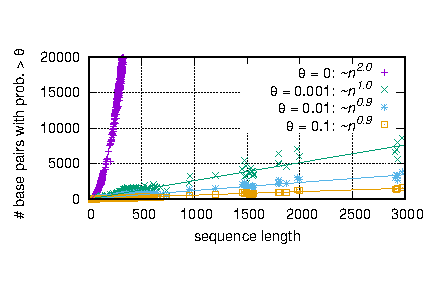
\includegraphics[width=.42\textwidth]{figs/Vienna_RNAfold_num_pij_curves.pdf}\\
\caption{
aaa
\label{bp-number}}
\end{figure}

% Secondary structure prediction problem, 
% though still difficult, 
% is well-defined in mathematics formation, and can be suitable modeled with the decomposable substructures. 
% Utilizing this decomposable nature, 
RNA secondary structure prediction is NP-complete \cite{Pedersen+:2000},
but nested (i.e., pseudoknot-free) secondary structures can be predicted with
cubic runtime dynamic programming algorithm. 
% based on an important paradigm free energy minimization 
Commonly, the minimum free energy (MFE) 
structure is predicted \cite{nussinov+jacobson:1980, zuker+stiegler:1981}.
% when a single structure is expected.
% and some prediction systems based on these algorithms, such as RNAstructure \cite{mathews+turner:2006}, \contrafold \cite{do+:2006} and \viennarnafold \cite{lorenz+:2011}, 
% have greatly improved the accuracy of prediction and are widely used.
% MEA -> partition function 
% For a given sequence, predicting the structure of minimum free energy (MFE) under certain free energy model by dynamic programming is a classical method for RNA secondary structure prediction. 
% cted.Free energy minimization is an important paradigm for predicting structure when a single structure is expe
% In the absence of many homologous sequences, the accuracy of MFE structure is 73\% in average \cite{mathews:2004}.
% However, this method assumes all thermodynamic parameters are correct and the energy model is perfect, which are both no the case in reality.
% Also, this method neglects the facts that multiple conformations exits at equilibrium \cite{mathews:2004}.
% This method 
% MFE method gives a practical solution to predict a single secondary structure, 
At equilibrium, the MFE structure is the most populated structure, 
however, 
% it neglects the fact that 
the MFE structure is a simplification because 
multiple conformations exist 
% at equilibrium 
as an equilibrium ensemble 
for RNA sequences \cite{mathews:2004}.
For example, many mRNAs {\textit {in vivo}} form a dynamic equilibrium and fold into a population of structures \cite{Long+:2007, Lu+:2008, Tafer+:2008, lai+:2018}. 
% as well as abandons all pseudoknotted structures.
% Many RNA sequences, for example mRNAs, exist in a thermodynamic ensemble of structures 
% \cite{lai+:2018}.%[53].
% As an alternative, partition function-based method \cite{mccaskill:1990} provides an ensemble of all pseudoknot-free structures, and based on it base pairing probabilities and structural entropy \cite{Huynen+} can be calculated.  
% As an alternative, 
Figure~\ref{Tebowned-RNA} shows the example of Tebowned RNA
which folds into more than one structure at equilibrium.
% ~\cite{Cordero+Das:2015}.
% TBWN-A, which has a long helices at 3'-end, 
% is the majority structure and accounts for $56 \pm 16\%$ of ensemble.
% While TBWN-B, which has two short helices at 5'-end, takes up $27 \pm 12\%$ of ensemble.
% Besides TBWN-A and TBWN-B illustrated in Figure~\ref{Tebowned-RNA}, Tebowned RNA can also fold into the state of TBWN-C 
% with a smaller ensemble proportion of $17 \pm 11\%$.
In this case, the prediction of one single structure, such as MFE structure, 
is not expressive enough to capture multiple states of Tebowned RNA %folding.
at equilibrim.

% Rather than predicting one single stucture, 
% partition function-based methods estimate the folding in a different point of view by
% taking into account ensemble of structures at equilibrium with Boltzmann Distribution.  
% Partition function, the sum of equilibrium constants for all possible secondary structures,
% is the normalization terms for calculating given secondary structure in the boltzmann ensemble.
Alternatively, we can compute the partition function, 
which is the sum of the equilibrium constants for all possible secondary structures,
and is the normalization term for calculating the probability of a secondary structure in the Boltzmann ensemble.
% Starting from the partition function,
% these methods are able to model mix of conformations,
% and further 
% we can % also
The partition function calculation can also be used to 
calculate base pairing probabilities of each nucleotide $i$ paired with each of possible nucleotides $j$~\cite{mccaskill:1990, mathews:2004}. 
% Base pairs with high probabilities 
% %in the matrix 
% indicate strong confidence of pairing in prediction,
% and are more likely to be paired in ground truth structures
% \cite{mathews:2004, Zuber+:2018}. 
% Figure~\ref{Tebowned-RNA}A 
The upper triangle in Figure~\ref{Tebowned-RNA}A presents the base pairing probability matrix of Tebowned RNA using \viennarnafold, 
showing that base pairs in TBWN-A have higher probabilities (in dark red) than
base pairs in TBWN-B (in light red).
This is consistent with the experimental result, i.e.,
TBWN-A is the majority structure that accounts for $56 \pm 16\%$ of the ensemble, 
while TBWN-B takes up $27 \pm 12\%$ of the ensemble~\cite{Cordero+Das:2015}.
% ~\cite{Cordero+Das:2015}.
% Besides producing base pairing probability matrix, 

In addition to model multiple states at equilibrim, 
base pairing probabilities are used for downstream prediction methods, 
such as maximum expected accuracy (MEA)~\cite{Knudsen+Hein:2003, do+:2006}, 
to assemble a structure with improved accuracy compared with the MFE structure \cite{lu+:2009}.
% As a by-product, the pair probabilities also enable maximum expected accuracy (MEA) structure prediction 
% \cite{do+:2006, lu+:2009}. % [29, 62].
Other downstream prediction methods, 
such as 
% HotKnot \cite{Ren+:2005}, % not based on partition function
ProbKnot~\cite{bellaousov+mathews:2010}, 
ThreshKnot~\cite{Zhang+:2019},
DotKnot~\cite{Sperschneider+Datta:2010} 
and IPknot~\cite{sato+:2011},
use base pairing probabilities to predict pseudoknotted structures with heuristics,
which is beyond the scope of standard cubic-time prediction algorithms.
Additionally, the partition function 
% can also be applied to do stochastic sampling based on the ensemble distribution
is the basis of stochastic sampling, 
in which structures are generated at random with their probability of occurring in the Boltzmann ensemble~\cite{ding+:2005, mathews:2006}.

% Moreover, although partition function-based method excluded pseudoknotted structures during dynamic programming process, 
% it is able to predict pseudoknotted base pairs and structure by using pair probability matrix, and pseudoknotted prediction systems such as HotKnot \cite{Ren+:2005}, ProbKnot \cite{bellaousov+mathews:2010}, DotKnot \cite{Sperschneider+Datta:2010} and IPknot \cite{Sato+:2011} all take pair probability matrix as inputs. 
% Figure~\ref{tRNA} compares MFE-based and partition function-based methods.
% Furthermore, single structure prediction based on partition function calculation, such as maximum expected accuracy (MEA) ThreshKnot \cite{do+:2006, threshknot}, achieves higher accuracy in average. 


% speed
Therefore, there has been a general shift from the classical MFE-based methods to partition function-based methods.
These methods, 
as well as the prediction engines based on them, such as partition function-mode of RNAstructure \cite{mathews+turner:2006}, 
\viennarnafold \cite{lorenz+:2011}, 
and \contrafold \cite{do+:2006}, 
suffer the slowness from their $O(n^3)$ runtime and scale poorly for longer sequences. 
The slowness of partition function-based methods is even more severe than the $O(n^3)$ MFE-based methods 
due to its much larger runtime constant factor.
For instance, for 
% {\it E.~coli} 
{\it H.~pylori} 23S rRNA (sequence length 2,968~{\it nt}), \viennarnafold %(version 2.4.11)
takes 8 seconds for the MFE structure prediction, 
but takes 36 seconds for partition function calculation 
and another 37 seconds for base pairing probabilities, 
which is in total $9 \times$ slower.
It is even worse for \contrafold,
which takes about 6 seconds for the MFE structure prediction,
but takes 50 seconds and 70 seconds for partition function and base pairing probabilities calculation, separately,
resulting to in total $20 \times$ runtime increase.
% 132.248859 contrafold

% , which is more than 9 $\times$ slower. 
% because function-based method takes two-round cubic loops for inside-outside calculation.

To alleviate the slowness issue, 
we present \linearpartition, 
which is inspired by the %efficient linearization idea of \linearfold \cite{huang+:2019}
recently proposed \linearfold algorithm \cite{huang+:2019} 
that approximates the MFE structure in linear time.
Using the same idea, \linearpartition can approximate
the partition function and base pairing probability matrix in linear time.
% Recently, \linearfold \cite{huang+:2019} 
% presents the first linear-time and linear-space MFE-based RNA folding prediction system.
% For the same 
% % {\it E.~coli} 
% {\it H.~pylori} 23S rRNA, \linearfold spends about 2 seconds, leading to a 4$\times$ runtime decrease.
% % Overall, \linearfold achieves significant efficiency and scalability improvement and higher accuracy. 
% % the first linear-time MFE-based (approximate) algorithm for RNA folding, 
% % achieves significant efficiency and scalability improvement and higher accuracy 
% % than classical $O(n^3)$ MFE-based method, especially on long sequences. 
% Inspired by the efficient linearization idea of \linearfold, we present \linearpartition, 
% which can approximate the partition function and base pairing probability matrix in linear time, 
% addressing speed bottleneck in existing systems.
% Similar as \linearfold, 
Like \linearfold,
\linearpartition % incrementally 
scans the RNA sequence from 5'-to-3'
using a left-to-right fashion dynamic programming
that runs in cubic time.
Unlike the classical bottom-up cubic-time McCaskill algorithm \cite{mccaskill:1990},
our left-to-right algorithm can apply the beam search pruning \cite{Huang+Sagae:2010} technique
to narrow down the search space, 
achieving linear-runtime in practice.
 % with substructure of lower energy.
% and only retain states with top $b$ free energy of ensemble (inside score), 
% where $b$ is the beam size.
% Though introducing beam prune to filter some structures,
Though the search is approximate,
the well-designed heuristic makes sure 
%that only states with worse ensemble free energy
the surviving structures capture the bulk of the free energy of ensemble,
and the resulting partition function is close to the exact version.  
%  (inside score) 
% are pruned,
% and partition function is still similar as optimal algorithm.
% and the majority is catched.

% \linearpartition, inherits efficiency and accuracy of \linearfold. 

% \linearpartition is 11$\times$ faster than \viennarnafold for the longest sequence ({\it H.~pylori} 23S rRNA, 2,968 nucleotides) in the ArchiveII dataset,
% and 256$\times$ faster for the longest sampled sequence (15,780 nucleotides) from RNAcentral that \viennarnafold can run.
\linearpartition is $2,771\times$ faster than \contrafold for the longest sequence (32,753~{\it nt})
% 32,767 nucleotides) 
that \contrafold can run 
in the dataset.
% Meanwhile, \linearpartition leads to a small improvement on PPV and Sensitivity compared with \viennarnafold.
% % in both MEA and ThreshKnot prediction 
% % using the probability matrix computed in linear time.
% Surprisingly, \linearpartition achieves higher accuracy improvement on longer families (16S and 23S rRNA).
Interestingly, \linearpartition is much faster without sacrificing accuracy when applied to downstream structure prediction tasks such as MEA and ThreshKnot (a thresholded version of ProbKnot), and even leads to a small accuracy improvement on longer families (small and large subunit rRNA).


% \begin{itemize}
% \item Present an alternative left-to-right dynamic programming fashion for partition function calculation.
% \item The first algorithm to achieve linear runtime and space for partition function and base pairing probability calculation.
% % \item . 
% \end{itemize}


